

\section{System purpose}

Everscalend is a DEFI (DEcentralized FInance) lending and borrowing system implemented on the Everscale Blockchain. Its main purpose is to provide Everscale users with a realiable way to lend and borrow cryptocurrency tokens. It makes it possible for users to generate profits on tokens they supply for lending and to acquire tokens by borrowing them instead of buying them.

\section{Terms of the system domain}

\begin{tabularx}{\linewidth}{|l|X|}
  \hline
  \multicolumn{1}{|c|}{\textbf{Term}} & \multicolumn{1}{c|}{\textbf{Definition}} \\\hline
  \endhead

  Interest rate & The rate of profit that is generated for the suppliers of tokens. The interest rates in Everscalend are algorithmically calculated and they increase when the borrowing demand increases and decrease when it decreases. \\\hline

  Reserve factor & Ranging from 0 to 1, it represents the portion of the interest rate that should be stored in the reserve whenever it is acquired. \\\hline

  Market & A pool of tokens of the same kind where all the tokens supplied by the users are stored. It also holds information like the exchange rate and reserve factor etc. \\\hline

  vToken & A virtual token, it is a currency that only exists on Everscalend and it is used to determine the amount of tokens that a supplier owns in a market. vTokens are acquired by the users when they supply some tokens to the market. When interest rate is accumulated on the supplied tokens to the market, the exchange rate from the vTokens to the real tokens increases to account for the accumulated interest that the suppliers will get to retrieve when they withdraw their tokens. \\\hline

  Collateral & An amount of vTokens that a borrower has to have in order to borrow some amount of real tokens that. Everscalend like other DEFI lending systems is over-collateralized which means that the collateral has to be worth more than the amount of tokens that will be borrowed. \\\hline

  Collateral factor & Ranging from 0 to 1, it represents the amount of tokens that can be borrowed for a collateral. e.g. a collateral factor of 0.9 allows the borrowing of a number of tokens worth $90\%$ of the collateral. \\\hline

  Account health & The sum of the USD value of a user's supplied tokens divided by the sum of the USD value of all the tokens they borrowed. It is used to determine whether a user is eligible for liquidation or not. When the account health is greater than one, we say that the user's account is healthy, otherwise it is unhealthy. \\\hline

  Liquidation & The process in which some user's debt is liquidated by another user, by paying a portion of the owed tokens in exchange for the borrower's vTokens at a better exchange rate than the market. \\\hline

  Liquidation Multiplier & A value superior to 1. It is the amount by which the amount of vTokens that the liquidator should get by market price is multiplied to increase the amount they really get. \\\hline

  Index & Refers to the interest rate index, which is a value that captures the history of interest rates of a market. It is updated after each transaction to compound the interest since the previous index. \\\hline
\end{tabularx}

\newpage
\section{Mathematical notations}
\label{spec:mn}
The following mathematical notations are used in the document to simplify the equations.

\newcommand\USD{\mathit{USD}}

\newcommand\M[1]{\mathit{m_{#1}}}
\newcommand\T[1]{\mathit{T_{#1}}}
\newcommand\vT[1]{\mathit{vT_{#1}}}

\newcommand\ER[2]{\mathit{ER(#1, #2)}}

\newcommand\BA[1]{\mathit{Ba(#1)}}
\newcommand\C[1]{\mathit{C(#1)}}

\newcommand\UR[1]{\mathit{UR_{#1}}}
\newcommand\UMul[1]{\mathit{UM_{#1}}}
\newcommand\UBR[1]{\mathit{UbR_{#1}}}
\newcommand\BIR[1]{\mathit{BIR_{#1}}}
\newcommand\RF[1]{\mathit{RF_{#1}}}

\newcommand\RTB[1]{\mathit{rTB(#1)}}
\newcommand\VTB[1]{\mathit{vTB_{#1}}}
\newcommand\RES[1]{\mathit{Res_{#1}}}

\newcommand\CF[1]{\mathit{CF(#1)}}
\newcommand\LMul[1]{\mathit{LMul(#1)}}
\newcommand\AH[1]{\mathit{AH_{#1}}}
\newcommand\BC[1]{\mathit{BC_{#1}}}
\newcommand\SI[1]{\mathit{SI_{#1}}}
\newcommand\BI[1]{\mathit{BI_{#1}}}
\newcommand\uvTA[2]{\mathit{uvTA_{#1, #2}}}


\newcommand\IND[2]{\mathit{Ind_{#1, #2}}}
\newcommand\INDL[1]{\mathit{Indl_{#1}}}
\newcommand\AI[1]{\mathit{AI_{#1}}}
\newcommand\SIF[1]{\mathit{SIF_{#1}}}

\begin{tabularx}{\linewidth}{|l X|}\hline
  $\M{T}$: & A market for tokens of type $T$. \\\hline
  $\vT{T}$: & Type of vToken that have $T$ as an underlying token. \\\hline

  $\ER{\T{1}}{\T{2}}$: & Exchange rate from the token $\T{1}$ to the token $\T{2}$, aka the $x$ in: $1\ \T{1} = x \T{2}$. \\\hline

  $\BA{m}$: & Borrowed amount of tokens in a market $m$. \\\hline
  $\C{m}$: & Amount of cash in a market $m$. \\\hline

  $\UR{m}$: & Utilization ratio of the market $m$. \\\hline
  $\UMul{m}$: & Utilization multiplier of the market $m$. \\\hline
  $\UBR{m}$: & Utilization base rate of the market $m$. \\\hline
  $\BIR{m}$: & Borrowing interest rate of the market $m$. \\\hline
  $\RF{m}$: & Reserve factor of the market $m$. \\\hline

  $\RTB{m}$: & Real token balance of the market $m$. \\\hline
  $\VTB{m}$: & vToken balance of the market $m$. \\\hline
  $\RES{m}$: & Amount of tokens stored in the reserves of the market $m$. \\\hline

  $\CF{T}$: & Collateral factor for a token T. \\\hline
  $\LMul{T}$: & Liquidation multiplier of the market $m$. \\\hline
  $\AH{u}$: & User's account health. \\\hline
  $\BC{u}$: & User's borrowing capacity. \\\hline
  $\SI{u}$: & User's supply information. \\\hline
  $\BI{u}$: & User's borrowing information. \\\hline
  $\uvTA{u}{T}$: & Amount of vTokens that a user $u$ owns which have as an underlying token $T$. \\\hline

  $\IND{m}{n}$: & $n$th interest rate index of the market $m$. \\\hline
  $\INDL{m}$: & Latest interest rate index of the market $m$. \\\hline
  $\SIF{m}$: & Simple interest factor of the market $m$. \\\hline
  $\AI{m}$: & Accumulated interest of the market $m$. \\\hline

\end{tabularx}
\newpage
\section{System functioning}

the Everscalend system uses markets, which are pools of fungible tokens with algorithmically calculated interest rates, based on the supply and borrow demand for the tokens they hold. Each market is unique to a cryptocurrency, and contains a transparent and publicly-inspectable ledger, with a record of all transactions and historical interest rates.

The lenders and the borrowers of tokens interact directly with the system, earning and paying a variable interest rate, without having to negotiate terms such as the interest rate or the value of collateral with a peer or counterparty.

In this section we describe the functioning of the system.

\subsection{Kinds of users}

There are two kinds of clearly identifiable users:
\begin{itemize}
  \item The admin who is the deployer of the main contracts of the system like \verb|MarketAggregator|, \verb|WalletController| or \verb|Oracle|.
  \item The ``normal'' users who interact with the system.
\end{itemize}
And there are four roles\footnote{\href{https://github.com/SVOIcom/everscalend-contracts/blob/8d24e268f9c44bd3e896fb6a28bbf8a42c7027a9/smart-contracts/src/utils/interfaces/IRoles.sol\#L13-L15}{From ``IRoles.sol'', Lines: 13-15.}} that can be taken by the users and which determine their permissions when it comes to interacting with the system:
\begin{itemize}
  \item Owner: this is the role of the admin only. It gives them the right to modify all the parameters of the system.
  \item Upgrader: this role can be given to a user by the owner and it gives them the right to upgrades some contracts' codes.
  \item Parameter changer: this role can be given to a user by the owner and it gives them the to modify some of the parameters of the system.
  \item Other: this is the role of all the users who don't have a privileged role and can only interact with the system to realise the market opeartions (supply, borrow ...) without being able to manually change the parameters of the system.
\end{itemize}

\subsection{User capabilities}

In this section we describe what the users can do by using the system.

\subsubsection{Supply}

A user that wishes to make a certain amount of their tokens available for borrowing has to supply them to the system. The supplied tokens are then aggregated to the tokens of the same kind that were supplied by other users.

The supplier receives vTokens for their supply that they can use as collateral to borrow other tokens. vTokens are a currency used to represent how many of the real tokens in the market a user can withdraw, they also determine how many he can borrow of other tokens.

\subsubsection{Withdraw}

A user who owns vTokens can pay with them to withdraw the tokens he supplied. The user can do it at any time provided that their account is healthy, aka $\AH{u} > 1$ with $\AH{u}$ being the user $u$ account health

\subsubsection{Borrow}
To borrow a certain amount of some token:

\begin{itemize}
  \item There have to be enough tokens in the market for the borrowing.
  \item The borrowed amount has to be within the user's borrowing capacity, noted $\BC{u}$ with $u$ being the user.
\end{itemize}

$\BC{u}$ represents the amount of vTokens that the user can still use as collateral to borrow. Once that amount is reached, the user can no longer perform any action that requires them to have free vTokens like borrowing or withdrawing.

\subsubsection{Repay}

A borrower can repay the amount they borrowed by returning it to the market. By doing that the collateral they set for the borrowing is freed and can be used to borrow other tokens.

\subsubsection{Liquidate}
% is the repetition necessary?
When a user's account is unhealthy, aka ($AH_u < 1$), the liquidation of his debt becomes possible. The liquidation process consists of selling the borrower's collateral vTokens at a discount in exchange for the repayment of the borrower's debt or a portion of it.

The purpose of this mecanism is to financially incentivize the liquidators to add liquidity to the system and pay other users' debts.

\subsection{Key system algorithms}

\subsubsection{Interest acquisition}

The values of interest rates increase when the demand is high and decrease when it is low. The calculation of the real interest requires some intermediary variables:

\begin{itemize}
  \item The utilisation rate\footnote{\href{https://github.com/SVOIcom/everscalend-contracts/blob/8d24e268f9c44bd3e896fb6a28bbf8a42c7027a9/smart-contracts/src/Market/libraries/MarketOperations.sol\#L16}{From ``MarketOperations.sol'', Line: 16.}} $\UR{m}$ for the market $m$:
  $$
    \UR{m} = \frac{ \BA{m} }{ \RTB{m} + \BA{m} }
  $$
  The utilisation rate unifies supply and borrowing demand into a single variable.
  \item The borrowing interest rate\footnote{\href{https://github.com/SVOIcom/everscalend-contracts/blob/8d24e268f9c44bd3e896fb6a28bbf8a42c7027a9/smart-contracts/src/Market/libraries/MarketOperations.sol\#L18-L19}{From ``MarketOperations.sol'', Lines: 18-19.}} $\BIR{m}$ for the market $m$:
  $$
    \BIR{m} = \UR{m} * \UMul{m} + \UBR{m}
  $$ % in: MarketOperations.calculateBorrowInterestRate
  \item the simple interest factor\footnote{\href{https://github.comdev/SVOIcom/everscalend-contracts/blob/8d24e268f9c44bd3e896fb6a28bbf8a42c7027a9/smart-contracts/src/Market/MarketsAggregator.sol\#L167}{From ``MarketOperations.sol'', Line: 167.}} $\SIF{m}$ for the market $m$:
  $$
    \SIF{m} = \BIR{m} \times \Delta t
  $$
\end{itemize}
The accumulated interest\footnote{\href{https://github.com/SVOIcom/everscalend-contracts/blob/8d24e268f9c44bd3e896fb6a28bbf8a42c7027a9/smart-contracts/src/Market/MarketsAggregator.sol\#L171-L172}{From ``MarketOperations.sol'', Lines: 171-172.}} for the market $m$ can then be calculated as follows:
$$
  \AI{m} = \BA{m} \times \SIF{m}
$$ % in: MarketsAggregator.finterestAccumulated
with $\Delta t$ being the time difference in seconds between the current time and the last moment at which the interest rate was calculated\footnote{\href{https://github.com/SVOIcom/everscalend-contracts/blob/8d24e268f9c44bd3e896fb6a28bbf8a42c7027a9/smart-contracts/src/Market/MarketsAggregator.sol\#L160}{From ``MarketOperations.sol'', Line: 160.}}.

\subsubsection{Interest rate indexes}

Each time the interest rate is calculated in a certain market, the interest rate index associated to that market is updated. New indexes are calculated\footnote{\href{https://github.com/SVOIcom/everscalend-contracts/blob/8d24e268f9c44bd3e896fb6a28bbf8a42c7027a9/smart-contracts/src/Market/MarketsAggregator.sol\#L165-L170}{From ``MarketsAggregator.sol'', Lines: 165-170.}} as follows:
$$
\IND{m}{n} = (\SIF{m} + 1) \times\IND{m}{n-1}
$$
With\footnote{\href{https://github.com/SVOIcom/everscalend-contracts/blob/8d24e268f9c44bd3e896fb6a28bbf8a42c7027a9/smart-contracts/src/Market/MarketsAggregator.sol\#L330}{From ``MarketsAggregator.sol'', Line: 330.}}: $\IND{m}{0} = 1$.

\subsubsection{Reserves}

When interest is accumulated, a portion of it, the size of which is determined by the reserve factor, is put in a reserve, the rest of it is stored as cash. After accumulating the interest, the reserve is updated by adding\footnote{\href{https://github.com/SVOIcom/everscalend-contracts/blob/8d24e268f9c44bd3e896fb6a28bbf8a42c7027a9/smart-contracts/src/Market/MarketsAggregator.sol\#L173-L175}{From ``MarketsAggregator.sol'', Lines: 173-175.}} $(\AI{m} \times \RF{m})$ to it.

The purpose of the reserves is to protect a portion of the lenders interest so that they don't lose everything in case of liquidation, only their cash can be liquidated. %reference code

\subsubsection{vToken exchange rate calculation}

As stated previously the exchange rates from vTokens to real tokens depend on the supply and borrowing demand of those tokens. It is calculated\footnote{\href{https://github.com/SVOIcom/everscalend-contracts/blob/8d24e268f9c44bd3e896fb6a28bbf8a42c7027a9/smart-contracts/src/Market/libraries/MarketOperations.sol\#L24-L26}{From ``MarketOperations.sol'', Lines: 24-26.}} as follows:

$$
  \ER{\vT{T}}{T} = \frac{\RTB{\M{T}} + \BA{m} - \RES{\M{T}}}{\VTB{\M{T}}}
$$

\subsubsection{Account health and borrow capacity calculation}

A user $u$'s account health determines whether or not it is liquidable, if $AH_u < 1$ then it is otherwise it isn't. If the user's account is liquidable then the user can't withdraw their tokens or borrow more tokens before some other users liquidiates them or they supply more tokens to the market to improve their account's health. The account's health is calculated whenever the user tries to perform any market operation or gets one of his loans liquidated.

\noindent Given\footnote{\href{https://github.com/SVOIcom/everscalend-contracts/blob/8d24e268f9c44bd3e896fb6a28bbf8a42c7027a9/smart-contracts/src/ModulesForMarket/interfaces/IModule.sol\#L203-L207}{From ``IModule.sol'', Lines: 203-207.}}:
$$
  sval(T, vTA) = \frac{vTA \times \ER{\vT{T}}{T}}{\ER{T}{\USD}} \times \CF{T}
$$
and\footnote{\href{https://github.dev/SVOIcom/everscalend-contracts/blob/8d24e268f9c44bd3e896fb6a28bbf8a42c7027a9/smart-contracts/src/ModulesForMarket/interfaces/IModule.sol\#L215-L226}{From ``IModule.sol'', Lines: 215-226.}}:
$$
  bval(\M{T}, ba, ind) =\begin{dcases}
    0 & ba = 0\\
    \frac{(ba \times ind)/ \INDL{\M{T}}}{\ER{T}{\USD}} & ba \neq 0 \wedge \INDL{\M{T}} \neq ind \\
    \frac{ba}{\ER{T}{\USD}} & ba \neq 0 \wedge \INDL{\M{T}} = ind
    \end{dcases}
$$
Where $\CF{T}$ is the collateral factor for the market of the tokens $T$. It is a value that is set by the adminitrator and which determines by how much the collateral has to be bigger than the borrowed amout.

The account health\footnote{\href{https://github.com/SVOIcom/everscalend-contracts/blob/8d24e268f9c44bd3e896fb6a28bbf8a42c7027a9/smart-contracts/src/ModulesForMarket/interfaces/IModule.sol\#L187-L227}{From ``IModule.sol'', Lines: 187-227.}} is then calculated as follows:
$$
  AH_u =
    \frac {
      \sum_{(\T{i}, \uvTA{u}{\T{i}}) \in \SI{u}}
        sval(\T{i}, \uvTA{u}{\T{i}})
    } {
      \sum_{(\M{\T{j}}, ba, ind) \in \BI{u}}
      bval(\M{\T{j}}, ba, ind)
    }
$$
Where:
\begin{itemize}
  \item $\SI{u}$: The supply information of the user $u$, which we represent as a collection of couples $(\M{\T{i}}, \uvTA{u}{\T{i}})$ with:
  \begin{itemize}
    \item $\T{i}$: the kind of the supplied token;
    \item $\uvTA{u}{\T{i}}$: the amount of vTokens that the user got from the supplying tokens of the type $\T{i}$.
  \end{itemize}
  \item $\BI{u}$: The borrow information of the user $u$, which we represent as a collection of triplets $(m_{T_j}, ba, ind)$ with:
  \begin{itemize}
    \item $\T{j}$: the kind of the borrowed token;
    \item $ba$: the amount that was borrowed;
    \item $ind$: the value of the interest rate index when the borrowing occured.
  \end{itemize}
\end{itemize}

A user's borrowing capacity\footnote{\href{https://github.com/SVOIcom/everscalend-contracts/blob/8d24e268f9c44bd3e896fb6a28bbf8a42c7027a9/smart-contracts/src/ModulesForMarket/BorrowModule.sol\#L98}{From ``BorrowModule.sol'', Line: 98.}} is a value in USD that determines how many vTokens a user can use as collateral or redeem, the limit being that the vToken's worth has to be less that the user's borrowing capacity. The borrowing capacity is calculated as follows:
$$
  \BC{u} = (\sum_{(m_{\T{i}}, \uvTA{u}{\T{i}}) \in \SI{u}} sval(\T{i}, \uvTA{u}{\T{i}})) - (\sum_{(m_{T_j}, ba, ind) \in \BI{u}} bval(m_{T_j}, ba, ind))
$$

\subsubsection{Liquidation}

The amount of vTokens the liquidator gets is calculated thanks to the liquidation multiplier $\LMul{\M{T}}$ which is the value by witch the amount of tokens they would get at market price is multiplied to increase it. If a liquidator wants to repay a portion $R_T$ of a borrower $lu$'s debt in tokens of type $T$, the amount of the borrower's vTokens that the liquidator will get $vTA$ is calculated\footnote{\href{https://github.dev/SVOIcom/everscalend-contracts/blob/8d24e268f9c44bd3e896fb6a28bbf8a42c7027a9/smart-contracts/src/ModulesForMarket/LiquidationModule.sol\#L118-L126}{From ``LiquidationModule.sol'', Lines: 118-126.}} as follows:
$$
  vTA = min(R_T \times \ER{T}{\vT{T}} \times \LMul{\M{T}}, \uvTA{lu}{T})
$$
Where $min$ is a function that returns the minimum of two values. The value of the liqudation multiplier is set manually by the admin.

\subsubsection{Module locking mecanism}

To avoid messing up with the pools of tokens and market parameters while a user is performing an operation, a locking mecanism is used, that prevents the modification of the data that is used during the user's operation. The locks are especially necessary when try to extract tokens from the markets by borrowing or withdarwing, or from other users through liquidation.

Such locks are used in:
\begin{itemize}
  \item \verb|BorrowModule|: The lock prevents other users from borrowing at the same time.
  \item \verb|LiquidationModule|: In this case the lock is on the liquidated user, the purpose is to prevent more than one user liquidating the same user's debt.
  \item \verb|WithdrawModule|: To prevent other users from withdrawing while one of them has started that process.
  \item \verb|UserAccount|: This conract uses two locks called \verb|borrowLock| and \\\verb|liquidationLock|. As their names suggest, \verb|borrowLock| locks the user's account during the processing of a borrow request, stopping the user from doing another one before the current one is finished. The \\\verb|liquidationLock| stops the user from withdarwing or borrowing while he is being liquidated.
\end{itemize}

\section{Architecture of the System}

\begin{figure}[h!]
  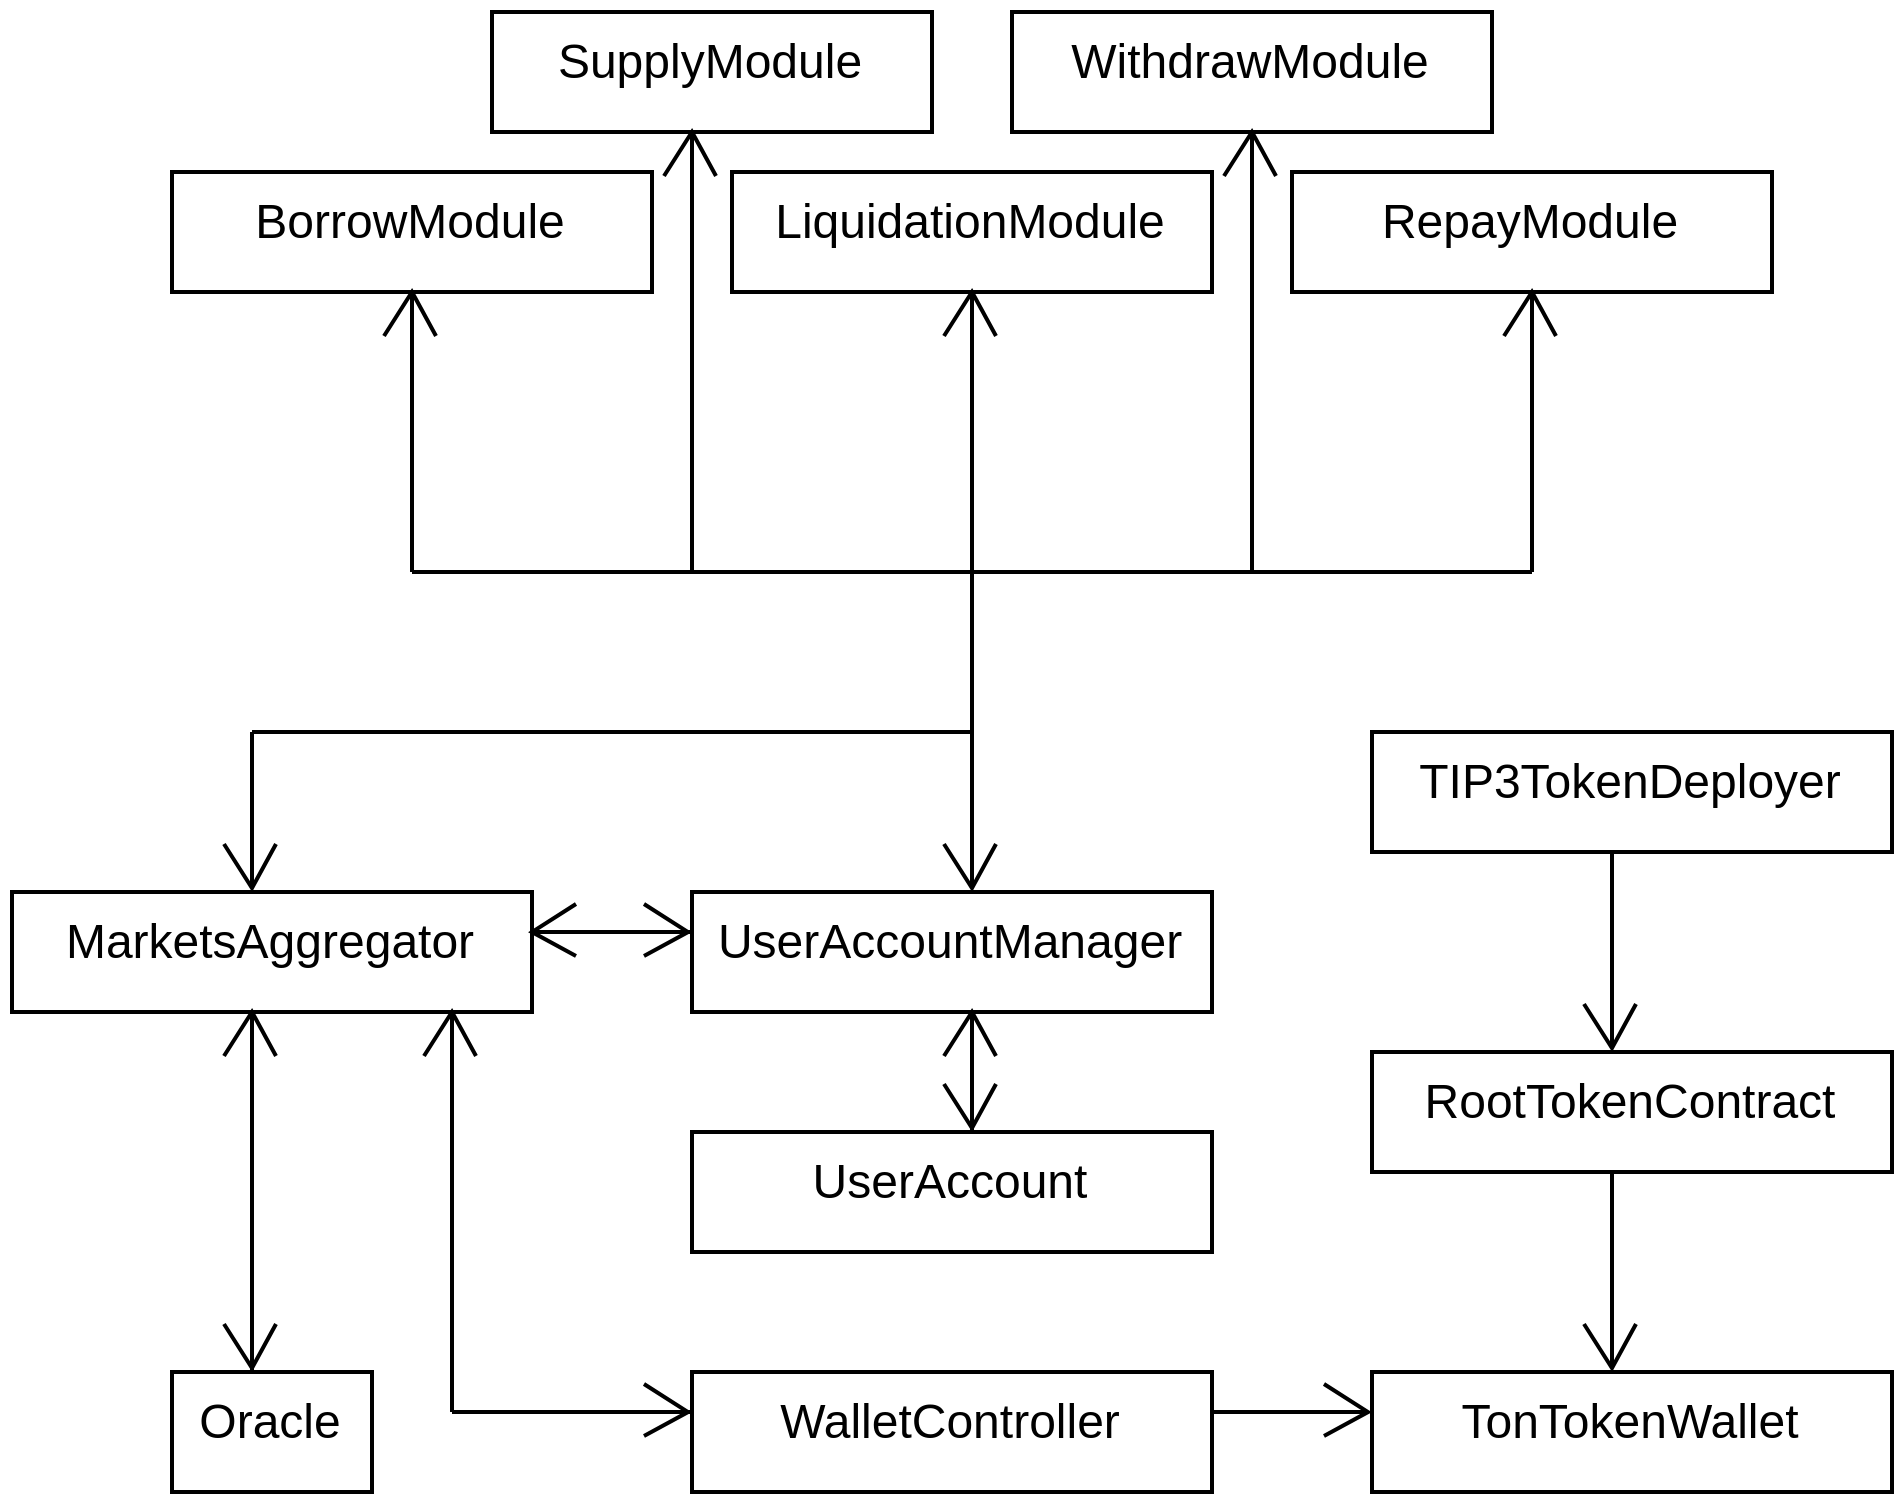
\includegraphics[width=\textwidth]{./assets/archi.png}
  \caption{System architecture with smart contract interactions}
  \label{fig:archi}
  \captionsetup[figure]{list=no} %So that it doesn't appear in list of figures
\end{figure}

Figure~\ref{fig:archi} shows a simplistic representation of the architecture of the system. The main smart contracts are shown with their names only while the interfaces, libraries and the smart contracts that are not necessary for comprehension were omitted. The smart contracts are connected with arrows which are meant to show interactions between them, these interactions will be described below.

\subsection{Main smart contracts}

\subsubsection{MarketsAggregator}

It mainly serves as a container for all the necessary information surrounding the markets, like the interest rates, the exchange rates and the borrow and supply amounts of each market.

\paragraph*{Functionalities:}
\begin{itemize}
  \item Adding and removing markets.
  \item Updating the information on the markets. As a result of market operations from users (like supplying, borrowing ... etc), changes in the prices of the supported tokens or market parameter modifications by the admin or privileged users.
\end{itemize}

\paragraph*{Interactions:}
\begin{itemize}
  \item Oracle: to get token price updates.
  \item Operations modules: to perform market operations.
  \item UserAccountManager: to update account health after performing operations.
  \item WalletController: to transfer tokens to(from?) when necessary.
\end{itemize}

\subsubsection{Operations modules}

These smart contracts are used to help perform the market operations by doing the necessary math for these operations.

\paragraph*{The smart contracts:}
\begin{itemize}
  \item SupplyModule
  \item WithdrawModule
  \item BorrowModule
  \item RepayModule
  \item LiquidationModule
\end{itemize}

\subsubsection{Oracle}

It is used by the MarketsAggregator smart contract to get price updates on the supported tokens in the markets.

\subsubsection{TonTokenWallet}

It serves as a TIP-3 token wallet and it handles token transfers to and from the wallet. Everscalend follows the TIP-3 token standard and these wallets are necessary to interact with the system. They can be delpoyed either by RootTokenContract or a user who has the address of the RootTokenContract associated to the wallet's token.

\paragraph*{Functionalities:}
\begin{itemize}
  \item Tranfer tokens to and from the wallet.
  \item Deploy a receiver's TonTokenWallet and transfer tokens to it.
  \item Burn tokens.
\end{itemize}

\subsubsection{RootTokenContract}

A contract that is deployed by a token owner and stores information about the root token (like its name, symbol and total supply).

\paragraph*{Functionalities:}
\begin{itemize}
  \item Minting tokens.
  \item Deploying instances of TonTokenWallet.
  \item Updating the information on the root token.
  \item Change root token owner.
\end{itemize}

\subsubsection{TIP3TokenDeployer}

it deploys RootTokenContract contracts.

\subsubsection{WalletController}

It's the smart contract that controls all the TIP-3 wallets of the markets and managers the operations that require token transfers to and from those wallets.

\paragraph*{Functionalities:}
\begin{itemize}
  \item Adding and removing market wallets.
  \item Getting information about market wallets.
  \item Decoding the payloads of messages that require TIP-3 token transfers and adds necessary information like message origin and token amount before passing them to MarketsAggregator.
  \item Allows the users to perform the supply, repay and liquidate operations.
\end{itemize}

\paragraph*{Interactions:}
\begin{itemize}
  \item MarketsAggregator: to communicate to it the details of the market operations that require TIP-3 token transfer into the wallets of the markets.
  \item TonTokenWallet: to transfer tokens a user's wallet.
\end{itemize}

\subsubsection{UserAccount}

It's used to store information about how a user interacts with the markets, like how much they borrowed from which market and how much they supplied to which market. It also allows the user to perform the borrow and withdraw operations.

It interacts only with UserAccountManager, which can request the information and to which it returns it.

\subsubsection{UserAccountManager}

UserAccountManager serves as an intermediary between the user, the UserAccount contract, the MarketsAggregator contract and the market operations modules.

\paragraph*{Functionalities:}
\begin{itemize}
  \item Deploys UserAccount contract.
  \item Handles requests and data transfers from MarketsAggregator and market modules to the UserAccount contract.
\end{itemize}

\paragraph*{Interactions:}
\begin{itemize}
  \item MarketsAggregator: to calculate user account health and perform market operations that were requested by the user.
  \item market modules: to perform market operations.
  \item UserAccount: to get user information and to update it.
\end{itemize}

\subsection{User interactions}

The users mainly interact with TonTokenWallet and UserAccount to perform the market operations mentioned previously. The operations in which the users have to request tokens are done through the UserAccount (withdraw, borrow) smart contract, while the operations in which the users have to send tokens are done through TonTokenWallet (supply, repay, liquidate). % are we sure that those are not done directly through WalletController?

\section{Usage scenarios}

This section contains low level descriptions of usage scenarios which describe how the users interatct with the smart contracts and how the smart contracts interact between them.
\newpage
Used notation:

\begin{tabularx}{\textwidth}{|l X|l X|} \hline
  UA: & UserAccount &         UAM: & UserAccountManager \\\hline
  MA: & MarketsAggregator &   WC: & WalletController \\\hline
  TTK: & TonTokenWallet &     SM: & SupplyModule \\\hline
  WM: & WithdrawModule &      BM: & BorrowModule \\\hline
  RM: & RepayModule &         LM: & LiquidationModule \\\hline
\end{tabularx}

In the source code a lot of the interactions between the smart contracts are done with the intermediary of interfaces. In these usage scenarios we ignore the interfaces and present only the interactions between the contracts which the interfaces refer to.

\subsection{Updating a user's account health}
We start with a "sub-scenario" which is the one of updating the user's account health. This scenario was added because it's used by the other ones and to avoid repeating it everytime, we describe here what happens when we that the user's account health is updated.

\begin{enumerate}
  \item \verb|UAM.calculateUserAccountHealth| is called from |UA| with a payload.
  \item \verb|UAM.calculateUserAccountHealth| calls \\\verb|MA.calculateUserAccountHealth| which:
  \begin{enumerate}[label*=\arabic*.]
    \item Updates the markets' information and calculates the user's account health.
    \item If the user's account is unhealthy a \verb|LiquidationPossible| event is emitted.
    \item A call is made to \verb|UAM.updateUserAccountHealth| with the new account health.
  \end{enumerate}
  \item \verb|UAM.updateUserAccountHealth| calls \verb|UA.updateUserAccountHealth| \\which calls, depending on the operation code provided in the payload, either \verb|UAM.requestTokenPayout|, \verb|UAM.returnAndSupply| or transfers the remaining gas to a povided address.
\end{enumerate}

\subsection{Supply}
\begin{enumerate}
  \item The user makes an internal transfer through \verb|TTK.internalTransfer| with a payload containing the supply operation code.
  \item The payload with information about the token wallet is passed to \\\verb|WC.tokensReceivedCallback|.
  \item The payload is decoded and after checking the operation code a call is made to \verb|MA.performOperationWalletController| with the necessary information about the supply operation.
  \item \verb|MA.performOperationWalletController| calls the Oracle to request the newest token prices, the response is receive with \\\verb|MA.receiveAllUpdatedPrices| which updates all the prices in the markets and calls \verb|MA.performOperation|.
  \item \verb|MA.performOperation| calls \verb|SM.performAction| which:
  \begin{enumerate}[label*=\arabic*.]
    \item Calculates the amount of vTokens to provide the user.
    \item Builds a data structure with the changes to the market (market delta) to which the supply was made.
  \end{enumerate}
  \item The market delta is sent to \verb|MA.receiveCacheDelta| which updates market informations and calls \verb|SM.resumeOperation| with the new market information.
  \item The information about the supply operation is then sent to \\\verb|UAM.writeSupplyInfo| which transfers it to \verb|UA.writeSupplyInfo|.
  \item \verb|UA.writeSupplyInfo| calls \verb|UAM.calculateUserAccountHealth| with a \\payload having the \verb|NO_OP| operation code.
  \item After updating account health, the remaining gas is transferred back to the supplier.
\end{enumerate}

\subsection{Withdraw}
\begin{enumerate}
  \item The user calls \verb|UA.withdraw| with the address of their TIP-3 wallet, the ID of the market to which their supplied their tokens and the amount their wish to withdraw.
  \item \verb|UA.withdraw| calls \verb|UAM.requestWithdraw| with the withdrawal information.
  \item \verb|UAM.requestWithdraw| calls \verb|MA.performOperationUserAccountManager| with the withdraw operation code.
  \item \verb|MA.performOperationUserAccountManager| calls the Oracle to request the newest token prices, the response is receive with \\\verb|MA.receiveAllUpdatedPrices| which updates all the prices in the markets and calls \verb|MA.performOperation|.
  \item \verb|MA.performOperation| calls \verb|WM.performAction|.
  \item \verb|WM.performAction| locks the module \verb|WM| and requests from \verb|UAM| the user's borrow and supply information which is provided by \verb|UA| and goes through \verb|UAM.receiveWithdrawInfo| which sends it to \\\verb|WM.withdrawTokensFromMarket|.
  \item \verb|WM.withdrawTokensFromMarket| checks that:
  \begin{itemize}
    \item The user's account is healthy.
    \item The user supplied at least as many tokens as the amount that they wish to withdraw.
    \item The worth in USD of the user's free collateral is equal or greater than the worth in USD of the amount of tokens they wish to withdraw.
  \end{itemize}
  Then calls \verb|MA.receiveCacheDelta| with the withdrawal information.
  \item \verb|MA.receiveCacheDelta| updates market information and calls \\\verb|WM.resumeOperation| with the new market information.
  \item \verb|WM.resumeOperation| unlocks the module \verb|WM| and sends the withdrawing information to \verb|UAM.writeWithdrawInfo| \\which calls \verb|UA.writeWithdrawInfo| which:
  \begin{enumerate}[label*=\arabic*.]
    \item updates the user's supply information by decreasing it with the withdrawn amount.
    \item builds a payload with the amount of tokens that need to be sent, the user's TIP-3 wallet address and the opeartion code \\\verb|REQUEST_TOKEN_PAYOUT|.
  \end{enumerate}
  \item A call is made to \verb|UAM.calculateUserAccountHealth| with the user's new supply and borrow information.
  \item After the user's account health is updated, \verb|UAM.returnAndSupply| is \\called.
  \item \verb|UAM.returnAndSupply| calls \verb|MA.requestTokenPayout| and \verb|WM.unlock| \\(which does nothing because the module was unlocked during the call to \verb|WM.resumeOperation|).
  \item \verb|MA.requestTokenPayout| calls \verb|WC.transferTokensToWallet| which calls \verb|WC.transfer|.
  \item \verb|WC.transfer| calls \verb|TTK.internalTransfer| which updates the user's balance with the amount of tokens that he requested to withdraw.
\end{enumerate}

\subsection{Borrow}
\begin{enumerate}
  \item The user calls \verb|UA.borrow| with the address of their TIP-3 wallet, the ID of the market from which they wish to borrow and the amount of tokens they wish to borrow.
  \item \verb|UA.borrow| locks the user account and calls \verb|UAM.requestIndexUpdate| with the borrowing information.
  \item \verb|UAM.requestIndexUpdate| calls \\\verb|MA.performOperationUserAccountManager| with the \verb|BORROW_TOKENS| operation code.
  \item \verb|MA.performOperationUserAccountManager| calls the Oracle to request the newest token prices, the response is receive with \\\verb|MA.receiveAllUpdatedPrices| which updates all the prices in the markets and calls \verb|MA.performOperation|.
  \item \verb|MA.performOperation| calls \verb|BM.performAction|.
  \item \verb|BM.performAction| locks the module \verb|BM| and requests from \verb|UAM| to update the market's indexes which is done by calling \verb|UA.borrowUpdateIndexes|.
  \item \verb|UA.borrowUpdateIndexes| gets from the markets the updates indexes and passes them along with the user's borrow and supply into to \\\verb|UAM.passBorrowInformation| which calls \verb|BM.borrowTokensFromMarket|.
  \item \verb|BM.borrowTokensFromMarket| checks that:
  \begin{itemize}
    \item That there are enough tokens in the market for the borrowing.
    \item That the user's account is healthy.
    \item That the user has enough collateral to make the borrowing.
  \end{itemize}
  \item A \verb|TokenBorrow| event is emitted with the borrowing information.
  \item \verb|BM.borrowTokensFromMarket| calls \verb|MA.receiveCacheDelta| with the borrowing information and the information about the changes to the market after the borrowing.
  \item \verb|MA.receiveCacheDelta| updates the market information and calls \\\verb|BM.resumeOperation| with the new market information.
  \item \verb|BM.resumeOperation| unlocks the module \verb|BM| and sends the borrowing information to \verb|UAM.writeBorrowInformation| which calls \\\verb|UA.writeBorrowInformation| which:
  \begin{enumerate}[label*=\arabic*.]
    \item Updates market information and the user's borrowing information.
    \item Unlocks \verb|UA|.
    \item Builds a payload with the \verb|REQUEST_TOKEN_PAYOUT| operation code.
  \end{enumerate}
  \item \verb|UAM.calculateUserAccountHealth| is called with the payload as well as the user's supply and borrow information.
  \item After the user's account health is updated, \verb|MA.requestTokenPayout| is called.
  \item \verb|MA.requestTokenPayout| calls \verb|WC.transferTokensToWallet| which calls \verb|WC.transfer|.
  \item \verb|WC.transfer| calls \verb|TTK.internalTransfer| which updates the user's balance with the amount of tokens that they borrowed.
\end{enumerate}

\subsection{Repay}
\begin{enumerate}
  \item The user makes an internal transfer through \verb|TTK.internalTransfer| with a payload containing the repay operation code.
  \item The payload with information about the token wallet is passed to \\\verb|WC.tokensReceivedCallback|.
  \item The payload is decoded and after checking the operation code a call is made to \verb|MA.performOperationWalletController| with the necessary information about the supply operation.
  \item \verb|MA.performOperationWalletController| calls the Oracle to request the newest token prices, the response is receive with \\\verb|MA.receiveAllUpdatedPrices| which updates all the prices in the markets and calls \verb|MA.performOperation|.
  \item \verb|MA.performOperation| calls \verb|RM.performAction| which calls \\\verb|UAM.requestRepayInfo|.
  \item \verb|UAM.requestRepayInfo| calls \verb|UA.sendRepayInfo| which updates market information and transfers it with information about the user's TIP-3 wallet to \verb|UAM.receiveRepayInfo| which calls \verb|RM.repayLoan|.
  \item \verb|RM.repayLoan| calculates how much of the loan will be repayed and the changes to the markets after the repayment. A \verb|RepayBorrow| event is emitted with the repayment information. That information is then sent to \verb|MA.receiveCacheDelta| which updates market informations and calls \verb|RM.resumeOperation| with the new market information.
  \item \verb|RM.resumeOperation| calls \verb|UAM.writeRepayInformation| which transfers it to \verb|UA.writeRepayInformation|.
  \item \verb|UA.writeRepayInformation| calls \verb|UAM.calculateUserAccountHealth| \\with one of the two operation codes:
  \begin{itemize}
    \item \verb|REQUEST_TOKEN_PAYOUT| if there are leftover tokens after the repayment.
    \item \verb|NO_OP| otherwise.
  \end{itemize}
  \item After updating account health, if there are leftover tokens after the repayment, they are transferred to the user's TIP-3 wallet.
\end{enumerate}

\subsection{Liquidate}
\begin{enumerate}
  \item The user makes an internal transfer through \verb|TTK.internalTransfer| with a payload containing the liquidation operation code.
  \item The payload with information about the token wallet is passed to \\\verb|WC.tokensReceivedCallback|.
  \item The payload is decoded and after checking the operation code a call is made to \verb|MA.performOperationWalletController| with the necessary information about the liquidation.
  \item \verb|MA.performOperationWalletController| calls the Oracle to request the newest token prices, the response is receive with \\\verb|MA.receiveAllUpdatedPrices| which updates all the prices in the markets and calls \verb|MA.performOperation|.
  \item \verb|MA.performOperation| calls \verb|LM.performAction| which calls \\\verb|UAM.requestLiquidationInformation|.
  \item \verb|UAM.requestLiquidationInformation| calls \\\verb|UA.requestLiquidationInformation| which updates market's indexes \\and calls \verb|UAM.receiveLiquidationInformation| with the new indexes and the user's supply and borrow information.
  \item \verb|UAM.receiveLiquidationInformation| calls \verb|LM.liquidate| which:
  \begin{enumerate}
    \item Checks the account health of the user that is targeted for liquidation to check that it is still required.
    \item Selects the minimum between the provided amount of tokens for the liquidation and the borrowed amount by the targeted user as the liquidation amount.
    \item Calculates the USD value of the liquidation amount.
    \item Calculates the how many of the targeted user's collateral to seize.
    \item Emits a \verb|TokensLiquidated| event with the liquidation information, update the markets and the liquidated user's borrow information.
    \item Calls \verb|MA.receiveCacheDelta| which updates market informations and calls \verb|RM.resumeOperation| with the new market information.
  \end{enumerate}
  \item \verb|LM.resumeOperation| recovers the sent information and passes it to \\\verb|UAM.seizeTokens| which calls \verb|UA.liquidateVTokens|.
  \item \verb|UA.liquidateVTokens| updates the user's borrow and supply information and calls \verb|UAM.grantVTokens|.
  \item \verb|UAM.grantVTokens| calls \verb|UA.checkUserAccountHealth| on the target \\user's account and wallet addresses to check their account health. Also calls \verb|UA.grantVTokens|.
  \item \verb|UA.grantVTokens| checks the liquidator's account health and builds a payload with the operation code \verb|RETURN_AND_UNLOCK| to pass to the function that checks the user's account.
  \item Once the new user's account health is recovered \verb|UAM.returnAndSupply| is called.
  \begin{itemize}
    \item if there are leftover tokens after the liquidation then a call is made to \verb|MA.requestTokenPayout| with the tokens to return and the liquidator's TIP-3 wallet.
    \item A call is made to \verb|LM.unlock| to unlock it and return the remaining gas to the liquidator's wallet.
  \end{itemize}
  \item \verb|MA.requestTokenPayout| calls \verb|WC.transferTokensToWallet|.
  \item A call is then made to \verb|TTK.transfer| which calls \verb|TTK.internalTransfer| to update the user's balance by increasing it with the returned amount of tokens.
\end{enumerate}
